\documentclass[12pt]{article}
\usepackage[a4paper, margin=.30in]{geometry}
\usepackage{graphicx ,
            wrapfig,
            xcolor, 
            enumerate,
            amsmath,fontenc, mhchem  ,tcolorbox, chemfig, makecell
            }
\usepackage{multirow}
\newcommand\headerMe[2]{\noindent{}#1\hfill#2}
\renewcommand{\thesection}{\Roman{section}}

\author{Zakaria HAOUZAN}
\date{\today}

\begin{document}
% headers --------------
\headerMe{Matière : Physique-Chimie}{Professeur : Zakaria HAOUZAN}\\
\headerMe{Unité : Méthode de
contrôle de
l’évolution des
systèmes
chimiques }{Établissement : Lycée SKHOR qualifiant}\\
\headerMe{Niveau : 2BAC-SM-X}{Heure : 12H}\\

% ------Content ________
\begin{center}

  \Large{Leçon $N^{\circ} 11 $: \color{red} Réactions d'estérification et d'hydrolyse }
\end{center}

%\begin{wrapfigure}[10]{r}{0.5\textwidth}
%    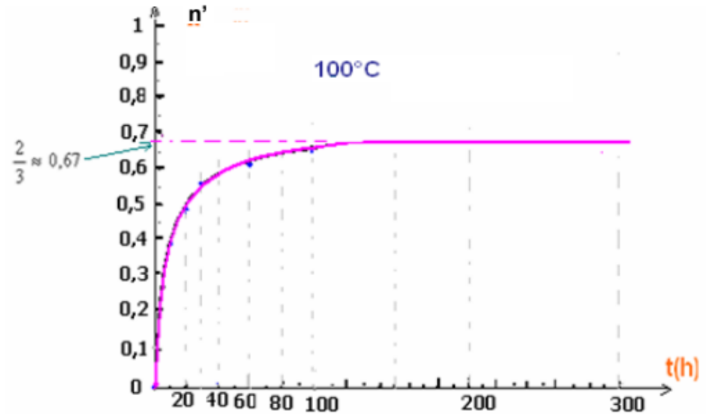
\includegraphics[width=0.5\textwidth]{./img/img00.png}
%\end{wrapfigure}

%\begin{wrapfigure}[10]{r}{0.5\textwidth}
%    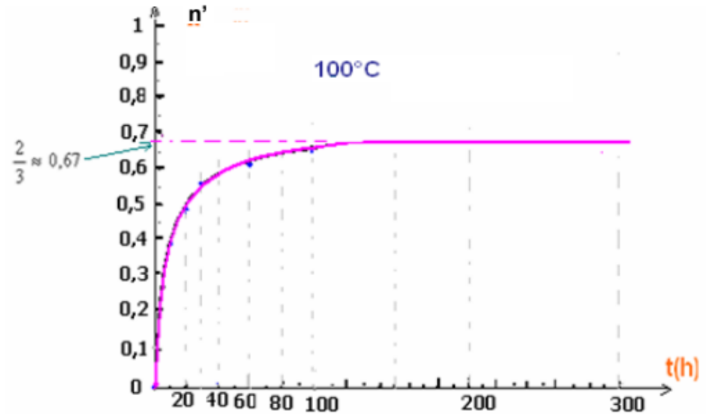
\includegraphics[width=0.5\textwidth]{./img/img00.png}
%\end{wrapfigure}



%\begin{tcolorbox}[colback=pink!10!white,
                  %colframe=blue!15!gray,
                  %title=Application -1- :
                 %]


  %\begin{wrapfigure}[10]{r}{0.3\textwidth}
  %\vspace{-2cm}
    %\includegraphics[width=0.3\textwidth]{./img/Mode_opératoire_dosage:.png}
%\end{wrapfigure}

\section{Rappel : }
\subsection{La chimie organique :}
La chimie organique s'appelle aussi la chimie du carbone car tous les composés organiques contiennent l'élément carbone C.
L'atome de carbone a pour numéro atomique $Z=6$ ,sa structure électronique est : $(K)^2(L)^4$
,il a quatre électrons dans la couche externe ,donc quatre électrons de valence , on dit qu'il est tétravalent

Dans tous les composés organiques l'atome de carbone ne participe que par quatre liaisons avec les atomes voisins.

\subsection{Les alcanes et les radicaux alkyls: }
Les alcanes sont des hydrocarbures saturés de formule brute générale $C_nH_{2n+2}$

 \begin{center}
    \begin{tabular}{ |c|c|c| } 
\hline
      \makecell{Nombre \\d'atome \\de Carbone} & \makecell{formule\\ brute} & \makecell{Nom de\\ l'alcane}\\\hline
      1 &$\ce{CH_4}$    & méthane\\\hline
      
      2 &$\ce{C_2H_6}$  & éthane\\\hline
      
      3 &$\ce{C_3H_8}$    &propane  \\\hline
                                                                         % -[1]-[-1]-[1]-[-1]
      4 &$\ce{C_4H_{10}}$ &butane \\\hline
      
      5 &$\ce{C_5H_{12}}$ &pentane \\\hline
      
      6 &$\ce{C_6H_{14}}$ &hexane\\\hline
      7 &$\ce{C_7H_{16}}$ &heptane\\\hline
      8 &$\ce{C_8H_{18}}$ &octane\\\hline
      9 &$\ce{C_9H_{20}}$ &nonane\\\hline
      10 &$\ce{C_10H_{22}}$ &décane\\\hline
      \hline
\end{tabular}
  \end{center}
 
  \begin{tcolorbox}
  Les radicaux alkyles ont pour formule brute $-C_n H_{2n+1}$
Le radical alkyl dérive d'un alcane par perte d'un atome d'hydrogène.

Le nom du radical alkyl s'obtient à partir du nom de l'alcane correspondant en remplaçant la terminaison "ane" par
"yle"
\end{tcolorbox}


\begin{center}
    \begin{tabular}{ |c|c|c|c|c| } 
\hline
      \makecell{Nombre \\d'atome \\de Carbone} & \makecell{formule\\ brute \\ de L'alcane} & \makecell{Nom de\\ l'alcane}&\makecell{L'alkyl \\correspondant} & \makecell{Son nom}\\
\hline
      1 &$\ce{CH_4}$    & méthane& $\ce{-CH_4}$ &  méthyle\\\hline
      
      2 &$\ce{C_2H_6}$  & éthane& $\ce{-C_2H_5}$ &  éthyle\\\hline
      
      3 &$\ce{C_3H_8}$    &propane & $\ce{-C_3H_7}$ & propyle \\\hline
                                                                         % -[1]-[-1]-[1]-[-1]
      4 &$\ce{C_4H_{10}}$ &butane& $\ce{-C_4H_9}$ &  butyle \\\hline
      
      \hline
\end{tabular}
  \end{center}

  \subsection{Nomenclature des alcanes ramifiés:}
  Le nom principal de l'alcane ramifié est donné par la chaine carbonée la plus longue que l’on le précède par les nom des
radicaux alkyls classés par ordre alphabétique et numérotés en utilisant les plus petits nombres possibes.

Exemples:

  \begin{center}
    \begin{tabular}{ |c|c|c| } 
\hline
      \makecell{Alcane ramifié } & \makecell{Son Nom } & \makecell{Sa formule \\topologique}\\
\hline
      
      $\chemfig{CH_3-CH(-[6]CH_3)-CH_2-CH_3}$ & 2-méthyle butane &  \chemfig{-[1](-[2])-[-1]-[1]-[-1] }  \\\hline
      
      $\chemfig{CH_3-C(-[6]CH_3)(-[2]CH_3)-CH_2-CH_3}$ & 2,2 diméthyle butane &  \chemfig{-[1](-[2])(-[-2.5])-[-1]-[1]-[-1] }  \\\hline

      $\chemfig{CH_3-CH(-[6]CH_3)-CH_2(-[2]CH_3)-CH_2-CH_3}$ & 2,3 diméthyle pentane &  \chemfig{-[1](-[2])-[-1](-[-2])-[1]-[-1] }  \\\hline
      
      $\chemfig{CH_3-CH(-[6]CH_3)-CH(-[2]C_2H_5)-CH_2-CH_3}$ & \makecell{3-éthyle \\2-méthyle pentane }&  \chemfig{-[1](-[2])-[-1](-[-2](-[5]))-[1]-[-1] }  \\\hline
      
      $\chemfig{CH_3-CH(-[6]CH_3)-C(-[2]CH_3)(-[-2]CH_3)-CH_2-CH(-[2]C_2H_5)-CH_2-CH_3}$ & \makecell{5-éthyle \\2,3,3-triméthyle heptane} &  \chemfig[angle increment=55]{-[1](-[2])-[-1](-[-2])(-[1.5])-[1]-[-1](-[5](-[5.5]))-[1]-[-1] }  \\\hline

      $\chemfig{CH_3-CH(-[6]CH_3)-CH(-[2]CH_3)-C(-[2]CH_3)(-[6]CH_4)-CH_2-CH_3}$ & \makecell{2,3,4,4 tétraméthyle\\ hexane} &  \chemfig[angle increment=55]{-[1]-[-1](-[4.9])-[1](-[2])-[-1](-[5])(-[5.5])-[1]-[-1] }  
      \\\hline
                     
           \hline
\end{tabular}
  \end{center}


  \section{Composés organiques oxygénés réaction d'estérification : }

  \subsection{Les alcools : }
  \subsubsection{Définition :}

La molécule d'alcool contient le groupement fonctionnel $-OH$ appelé groupement hydroxyle.

La formule brute générale des alcool :$R-OH$.

R- : est un groupe alkyl. $C_nH_{2n+1}$


\subsubsection{Nomenclature des alcools: }
Le nom de l'alcool se déduit du nom de l'alcane correspondant en remplaçant le (e) dans la terminaison du nom de l'alcane par (ol)

Exemple : 
méthane $CH_4$: méthanol $CH_3-OH$


éthane $C_2H6$ : éthanol $C_2H_5-OH$

Pour les aclcool ramifiés, la chaine carbonée principale est la plus longue chaîne qui comporte le carbone fonctionnel et pour préciser la position du groupe $-OH$ sur la chaîne carbonée on utilise le suffixe (ol) précédé du plus petit nombre qui indique la position du carbone fonctionnel sur la chaîne.



\subsection{Les acides carboxyliques:}
\subsubsection{Définition}
L’acide carboxylique est un composé organique dont la molécule possède le groupement fonctionnel
suivant :
\begin{center}
%\begin{wrapfigure}[10]{r}{0.5\textwidth}
	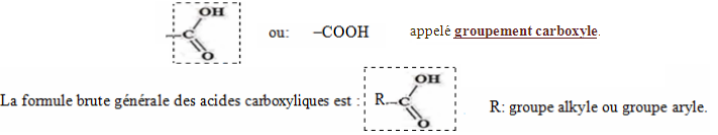
\includegraphics[width=0.5\textwidth]{./img/acideOique.png}
%\end{wrapfigure}

\end{center}



\subsubsection{Nomenclature des acides carboxyliques:}
Le nom de l'acide carboxylique se déduit de celui de l'alcane correspondant en remplaçant le (e) dans la terminaison du nom de l'alcane par (oique) que l'on fait précédé par le mot "acide"

Exemple : 

méthane : acide méthanoique $HCOOH$

éthane : acide éthanoique $CH_3-COOH$
\begin{tcolorbox}[colback=pink!10!white,
                  colframe=blue!15!gray,
                  title=Remarque  -1- :
                 ]
Dans le cas des acides carboxyliques on commence la numérotation à partir du carbone fonctionnel qui se trouve toujours au bout de la chaîne.


			 \end{tcolorbox}


\subsection{Anhydride de l'acide carboxylique:}
\subsubsection{Définition:}
La molécule de l'anhydride de l'acide carboxylique contient le groupement fonctionnel suivant:
\begin{center}
	$\chemfig{-C(=[6]H)-O-C(=[6]O)-}$ ou $\ce{-CO-O-CO-}$

\end{center}
La formule brute générale des anhydrides de l'acide carboxylique est :

$$\chemfig{R-C(=[::+60]O)-[::-60]O-[::-60]C(=[::+60]O)-[::-60]R}$$

\subsection{Préparation de l'ahydride de l'acide carboxylique:}

La préparation de l'anhydride de l'acide carboxylique se fait à partir de l'acide carboxylique par chauffage à $700^oC$
et en utilisant un déshydratant (comme l'oxyde de phosphore $P_4O_{10}$).

Pendant cette réaction il y'a élimination d'une molécule d'eau entre deux molécules d'acide.

\begin{center}
%\begin{wrapfigure}[10]{r}{0.5\textwidth}
	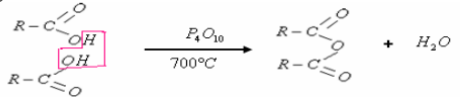
\includegraphics[width=0.5\textwidth]{./img/anydr.png}
%\end{wrapfigure}

\end{center}



Le nom de l'anhydride se dérive de celui de l'acide carboxylique correspondant en remplaçant le mot acide par
anhydride.

Exemples:

A partir de l'acide éthanoïque $CH_3-CO-OH$ on obtient l'anhydride éthanoïque $CH_3-CO-O-CO-CH_3$.

A partir de l'acide méthanoïque $HCO-OH$ on obtient l'anhydride méthanoïque $HCO-O-OCH$ .

A partir de l'acide éthanoïque $CH_3-CO-OH$ et l'acide méthanoïque $HCO-OH$ on obtient l'anhydride éthanoïque et
méthanoïque et $CH_3-CO-O-OCH$.


\subsection{Les esters:}
\subsubsection{Définition:}
Les esters sont des composés organiques, ce sont généralement des liquides volatils caractérisés par une odeur
agréable.
La molécule de l'anhydride de l'acide carboxylique contient le groupement fonctionnel suivant:

$$\chemfig{-C(=[::+60]O)-[::-60]O-C}$$

La formule brute générale des esters est :


$$\chemfig{R-C(=[::+60]O)-[::-60]O-R'}$$


\subsubsection{Nomenclature:}
Le nom de l'ester se compose de deux parties:

-La première partie se dérive du nom de l'acide correspondant en remplaçant la terminaison"oique" par "oate".

-La deuxième partie c'est le nom du radical alkyl -R' lié à l'atome d'oxygène.

Exemples: CH3-COO-CH2-CH2-CH2-CH3 éthanoate de butyle

$\chemfig{CH_3-C(-[2]CH_3)(-[6]CH_3)-C(=[::+60]O)(-[::-60]O-CH_3)}$
2,2-diméthylpropanoate de méthyle

$\chemfig{CH_3-C(=[::+60]O)(-[::-60]O-CH(-[6]CH_3)-CH_3)}$
éthanoate de 1-méthyléthyle


$\chemfig{CH_3-CH_2-C(-[2]CH_3)(-[6]CH_3)-C(=[::+60]O)(-[::-60]O-CH(-[6]CH_3)-CH_2-CH_3)}$
2,2-diméthylbotanoate de 1-méthylpropyle


\subsection{Réaction d'estérification:}
La Réaction d'un acide carboxylique avec un alcool conduit à la formation d'ester et d'eau. Cette réaction s'appele :Estérification.


$$\chemfig{R-C(=[::+60]O)-[::-60]O-H} + R'-OH \rightarrow \chemfig{R-C(=[::+60]O)-[::-60]O-R'} + H_2O$$


\section{Etude expérimentale de la réaction d'estérification : }

\subsection{Description de l'expérience de Berthelot:}

Cette étude a été réalisé par le chimiste français Berthelot en 1862 dont le protocole expérimental est le suivant:

Un mélange équimolaire constitué d'une mole d'éthanol $C_2H_5OH$ et une mole d'acide éthanoique $CH_3COOH$ est
repartie après homogénésation ,dans plusieurs tubes à essaies identiques scellées et placés à température constante
$100^{\circ}C$

Chaque tube contient : 60g donc 1 mole de $CH_3COOH$ et 46g donc 1 mole de $C_2H_5OH$


Dans chaque tube démarre l'estérification et les divers échantillons évoluent en parallèle, de façon identique.

Pour déterminer la nombre de moles d'ester formé à un instant t donné, on prélève un tube et on lui fait subir une
trempe dans glacée pour arrêter la réaction puis on dose l’acide présent (restant) dans le tube à cet instant t à l’aide d’une solution de soude de concentration connue.

-Si initialement on part de 1mole de CH3COOH et 1mole de $C_2H_5OH$ et si  '(n) est le nombre de moles de $CH_3COOH$ restant à l'instant t , n'=1-n : représente le nombre de moles de $CH_3COOH$ qui a réagit c'est à dire le nombre de moles
d'ester formé à l'instant t.

\begin{center}
	\begin{tabular}{|p{2.2cm} |p{2.2cm} |p{4cm} |c|} 
 \hline
 \multicolumn{4}{|c|}{ $CH_3COOH + C_2H_5OH \rightarrow CH_3COOC_2H_5 + H_2O$} \\ 
 \hline\hline
 1 & 1 & 0 & 0 \\ 
 \hline
 1-n' &	1-n' & n' & n' \\
 \hline
  \hline
\end{tabular}
\end{center}


\begin{center}
\begin{tabular}{||c|c|c|c|c|c|c|c|c|c|c|c|c||} 
 \hline
 t(h) &0&2&4&10&20&30&40&60&80&100&150&200\\ [0.5ex] 
 \hline
 n &1&0,82&0,74&0,62&0,51&0,44&0,42&0,39&0,38&0,64&0,34&0,34\\ [0.5ex] 
 \hline
 n' &0&0,181&0,26&0,38&0,49&0,56&0,58&0,61&0,62&0,64&0,66&0,66\\ [0.5ex] 


 \hline
 \hline
\end{tabular}
\end{center}


%\begin{wrapfigure}[10]{r}{0.5\textwidth}
\begin{center}
	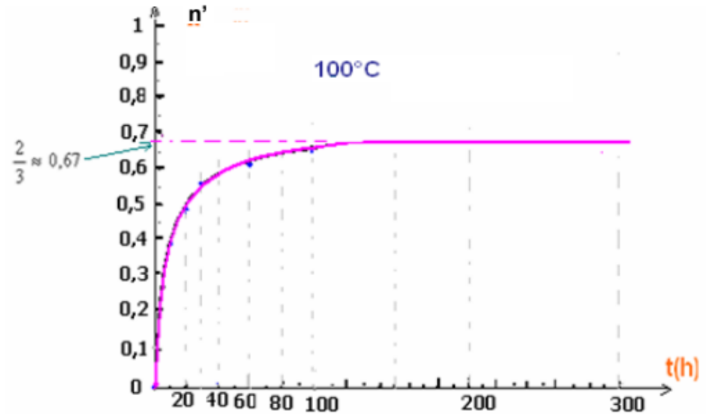
\includegraphics[width=0.5\textwidth]{./img/img00.png}
\end{center}
%\end{wrapfigure}



Pour obtenir un mélange de composition constante à 100oC , on a besoin de 150heures , donc la réaction d'estérification
est une réaction lente
A l'état final la composition du mélange devient constante mais aucun des réactifs n'a disparu donc la réaction d'estérification est
limitée. (En plus c’est une réaction endothermique)

\subsection{Caractéristiques de la réaction d'éstérification:}
La réaction d'estérification est une reaction lente , limitée et endothermique.
La limite de la réaction d'éstérification ne dépend que de la classe de l'alcool utilisé :

\begin{center}
\begin{tabular}{||c|c||} 
 \hline
 Classe de l'alcool &La limite\\ [0.5ex] 
 Alcool primaire &$67\%$\\ [0.5ex] 
 Alcool secondaire &$60\%$\\ [0.5ex] 
 Alcool tertaire &$5\%$\\ [0.5ex] 
 \hline
 \hline
\end{tabular}
\end{center}

\subsection{Les facteurs cinétiques de la réaction d'éstérification:}
\subsubsection{Infuence de la température:}
On donne les résultats de l'évolution d'un système équimolaire d'acide éthanoique et d'éthanol à différentes
températures.


%\begin{wrapfigure}[10]{r}{0.5\textwidth}
\begin{center}
	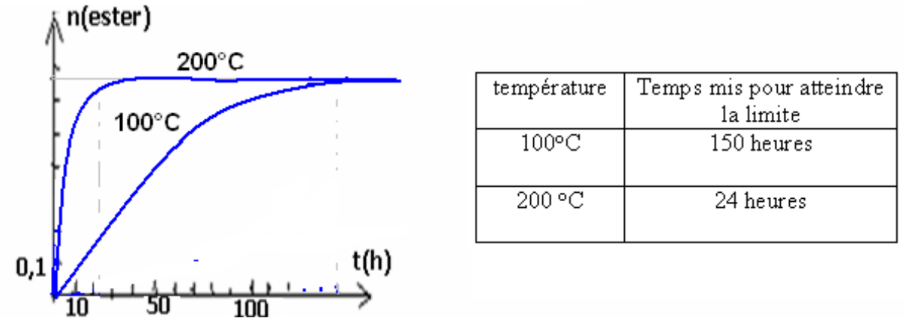
\includegraphics[width=0.5\textwidth]{./img/img01.png}
\end{center}
%\end{wrapfigure}



L'élévation de la température du milieu réactionnel augmente la vitesse de la réaction d'estérification sans influer sur
la limite de l'éstérification.

\subsubsection{Infuence du catalyseur:}

\section*{ Définition d'un catalyseur : }
Un catalyseur est une espèce chimique, introduite dans le milieu réactionnel, qui a pour effet d'augmenter la vitesse de réaction sans figurer dans l'équation de la réaction (voir dernier chapitre: la catalyse).

\section*{Catalyse des réactions d'estérification et d'hydrolyse de l'ester}

Les ions oxonium ($H3O^+$ ou plus simplement $H^+$) catalysent aussi bien la réaction d'estérification que la réaction inverse. Ils sont fréquemment introduits dans le milieu réactionnel par l'acide sulfurique ou l'acide paratoluènesulfonique.

Ce catalyseur permet d'atteindre plus rapidement l'état d'équilibre sans changer la composition du milieu réactionnel à l'équilibre.

\section{Etude expérimentale de la réaction d'hydrolyse:}
\subsection{Réaction d’hydrolyse:}
La réaction d'hydrolyse est la réaction entre l'ester et l'eau pour donner l'acide carboxylique est l'alcool c'est la réaction inverse
de la réaction d'estérification.

$$\chemfig{R-C(=[::+60]O)-[::-60]O-R'} + H_2O \rightarrow \chemfig{R-C(=[::+60]O)-[::-60]O-H} + R'_OH$$

\subsection{Etude de la réaction d'hydrolyse:}
En utilisant la même méthode utilisée dans l'étude de l'étérification ,on peut suivre l'évolution de la réaction d'yhdrolyse
en dosant l'acide formé par une base de concentration connue ce qui permet de tracer la courbe de la variation de la quantité de
matière d'ester restant en fonction du temps.
La courbe suivante représente la quantité de matière d'ester restant en fonction de temps.


\begin{center}
	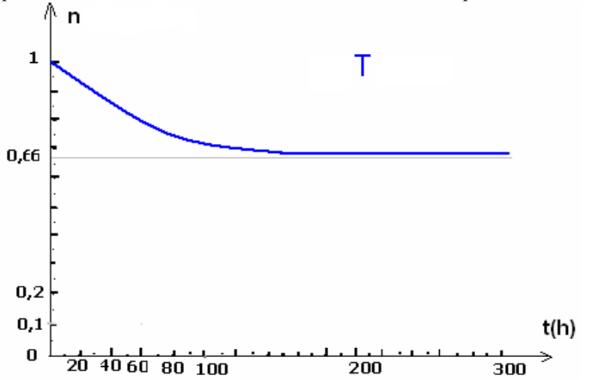
\includegraphics[width=0.3\textwidth]{./img/img02.png}
\end{center}

\begin{tcolorbox}
La réaction d'hydrolyse est une réaction lente ,limitée.(et endothermique)
\end{tcolorbox}

\section{Equilibre chimique : estérification hydrolyse}
\subsection{Les facteurs influençant l'équilibre : }
\subsubsection{Amélioration du rendement de l'estérification:}

Le calcul du rendement permet de déterminer l'efficacité d'une synthèse chimique de l'ester formé.
Or la réaction d'estérification est toujours accompagné de la réaction d'hydrolyse et ces deux réactions sont limitées, donc on a toujours $x_f< x_{max}$ .

Le rendement de la réaction d'estérification est égal au rapport de la quantité de matière du produit obtenue $n_{exp}$ par celle maximale attendue $x_{max}$ : $r = \frac{n_{exp}}{n_{max}}$

	\begin{tcolorbox}
Remarque: le rendement de l'estérification dépend de la classe de l'alcool utilisé :

Pour les alcools primaires r= 67\%

Pour les alcools secondaires r= 60\%

Pour les alcools tertiaires r= 5\%
	\end{tcolorbox}

\begin{center}
	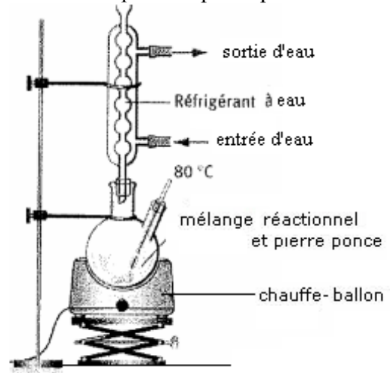
\includegraphics[width=0.3\textwidth]{./img/img03.png}
\end{center}
\begin{tcolorbox}[colback=pink!10!white,
                  colframe=blue!15!gray,
                  title=Remarque  -3- :
                 ]

 Généralement la température d'ébullition de l'ester est inférieure à celle des autres constituants du mélange
réactionnel , pour cela on utilise le chauffage à reflux qui a pour but

-Le chauffage du mélange réactionnel.

- Eviter de perdre une partie des réactifs et des produits par vaporisation.

			 \end{tcolorbox}

			 \subsubsection{ facteurs influençant l'équilibre:}
\begin{center}
\begin{tabular}{||c|c||} 
 \hline
 \makecell{Infuence sur la vitesse de la réaction\\d'estérification}&Infuence sur l'état final\\\hline 
 \makecell{ Le système chimique atteint son état\\d'équilibre plus
rapidement sans influer sur\\sa composition finale soit:\\-Par élévation de la température.
\\-En utilisant le catalyseur ($H_3O^+)$.}

																	&  \makecell{Pour déplacer l'équilibre dans le sens de la formation de \\l'ester et augmenter le rendement de l'estérification on doit
\\soit:
\\-éliminer l'un des produits : l’eau ou l’ester.
\\-Utiliser de l'un des réactifs(l'alcool ou l'acide) en excès..}\\  
 \hline
 \hline
\end{tabular}
\end{center}




\end{document}

